\documentclass[10pt,utf8,compress,xcolor=dvipsnames]{beamer}
\usefonttheme{professionalfonts}
\usepackage[greek,english]{babel}
%\usefonttheme{}
%\usetheme{Hannover}
\usetheme{Warsaw}
\usepackage{graphicx}
\usepackage{amsmath}
\usepackage{slashed}
\setbeamercolor{background canvas}{bg=white}
\setbeamertemplate{navigation symbols}{}
\usepackage{float}

\setbeamertemplate{headline}{}

\usepackage[absolute,overlay]{textpos}
\usepackage{rotating}
\usepackage{multicol}
\usepackage{ifthen}
\usepackage[dvipsnames]{xcolor}
\usepackage{tikz}


%Define color environments:

\newenvironment{DK}[1]{{\color{gray}Commend from D: #1}}

\newenvironment{DKnew}[1]{{\color{blue}NEW from D: #1}}

\newenvironment{DKres}[1]{{\color{BrickRed}RESTRUCTURED from D: #1}}




\newcommand{\dint}{  \displaystyle \int }
%%%%%%%%%%%%%%%%%%%%%%%%%%%%%%%%%%%%%%%%%%
\newcommand{\ie}{{\em i.e.} }
\newcommand{\eg}{{\em e.g.} }
\newcommand{\GeV}{{\rm GeV}}
\newcommand{\TeV}{{\rm TeV}}
\newcommand{\MeV}{{\rm MeV}}
\newcommand{\keV}{{\rm keV}}

\newcommand{\rhs}{RHS }
\newcommand{\lhs}{LHS }


\newcommand{\geff}{ g_{\rm eff} }
\newcommand{\heff}{ h_{\rm eff} }
 
\newcommand{\Ham}{ \mathcal{H} }
 
\newcommand{\thetamax}{ \theta_{\rm max}{} }

 
\newcommand{\thetai}{ \theta_{\rm ini}{} }

\newcommand{\fa}{ f_{\alpha}{} }
 
\newcommand{\ti}{ t_{\rm ini}{} }
 
\newcommand{\Ri}{ R_{\rm ini}{} }


\newcommand{\tosc}{ t_{\rm osc}{} }

\newcommand{\Omegai}{ \Omega_{\rm ini} }
 
\newcommand{\ma}{ m_\alpha{} }

\newcommand{\Lint}{ \mathcal{L}_{\rm int} }


\newcommand{\vev}[1]{\langle #1 \rangle}
\newcommand{\Bvev}[1]{\Bigg\langle #1 \Bigg\rangle}
\newcommand{\bvev}[1]{\Big\langle #1 \Big\rangle}




\newcommand{\lrb}[1]{\left( #1 \right)}
\newcommand{\lrsb}[1]{\left[ #1 \right]}
\newcommand{\lrBigb}[1]{\Big( #1 \Big)}
\newcommand{\lrBigsb}[1]{\Big[ #1 \Big]}
\newcommand{\lrBiggb}[1]{\Bigg( #1 \Bigg)}
\newcommand{\lrBiggsb}[1]{\Bigg[ #1 \Bigg]}

\newcommand{\lrBigcb}[1]{\Big\{ #1 \Big\}}
\newcommand{\lrBiggcb}[1]{\Bigg\{ #1 \Bigg\}}
%%%%%%%%%%%%%%%%%%%%%%%%%%%%%%%%%%%%%%%%%

%%%%%%%%%%%%%%%%%%%%%%%%%%%%%%%%%%%%%%%%%%%%%%%%%%%--Begin_refs--%%%%%%%%%%%%%%%%%%%%%%%%%%%%%%%%%%%%%%%%%%%%%%%%%%%%%%%%%%%%%%%%%%%%%%
\newcounter{NumArgs}

%Define reference to an arbitrary number of equations (\eqs{label_1,label_2....,label_n} will show eqs. ref_1, ref_2, ..., and ref_n)
\newcommand{\eqs}[1]{\setcounter{NumArgs}{0}\foreach\i in{#1}{\stepcounter{NumArgs}}%
\ifthenelse{\equal{\theNumArgs}{1}}{eq.~(\ref{#1})}%
{\ifthenelse{\equal{\theNumArgs}{2}}%
{eqs.~\foreach\i[count=\q]in{#1}{\ifthenelse{\equal{\q}{\theNumArgs}}{and (\ref{\i})}{(\ref{\i})~}}}%
{eqs.~\foreach\i[count=\q]in{#1}{\ifthenelse{\equal{\q}{\theNumArgs}}{and (\ref{\i})}{(\ref{\i}),~}}}}}


%Define reference to an arbitrary number of equations (\Eqs{label_1,label_2....,label_n} will show Eqs. ref_1, ref_2, ..., and ref_n)
\newcommand{\Eqs}[1]{\setcounter{NumArgs}{0}\foreach\i in{#1}{\stepcounter{NumArgs}}%
\ifthenelse{\equal{\theNumArgs}{1}}{Eq.~(\ref{#1})}%
{\ifthenelse{\equal{\theNumArgs}{2}}%
{Eqs.~\foreach\i[count=\q]in{#1}{\ifthenelse{\equal{\q}{\theNumArgs}}{and (\ref{\i})}{(\ref{\i})~}}}%
{Eqs.~\foreach\i[count=\q]in{#1}{\ifthenelse{\equal{\q}{\theNumArgs}}{and (\ref{\i})}{(\ref{\i}),~}}}}}


%Define reference to an arbitrary number of labels (\REF{label_1,label_2....,label_n} will show ref_1, ref_2, ..., and ref_n)
\newcommand{\refs}[1]{\setcounter{NumArgs}{0}\foreach\i in{#1}{\stepcounter{NumArgs}}%
\ifthenelse{\equal{\theNumArgs}{1}}{(\ref{#1})}%
{\ifthenelse{\equal{\theNumArgs}{2}}%
{\foreach\i[count=\q]in{#1}{\ifthenelse{\equal{\q}{\theNumArgs}}{and (\ref{\i})}{(\ref{\i})~}}}%
{\foreach\i[count=\q]in{#1}{\ifthenelse{\equal{\q}{\theNumArgs}}{and (\ref{\i})}{(\ref{\i}),~}}}}}



%Define reference to an arbitrary number of figs (\Figs{label_1,label_2....,label_n} will show ref_1, ref_2, ..., and ref_n)
\newcommand{\Figs}[1]{\setcounter{NumArgs}{0}\foreach\i in{#1}{\stepcounter{NumArgs}}%
\ifthenelse{\equal{\theNumArgs}{1}}{Fig.~(\ref{#1})}%
{\ifthenelse{\equal{\theNumArgs}{2}}%
{Figs.~\foreach\i[count=\q]in{#1}{\ifthenelse{\equal{\q}{\theNumArgs}}{and (\ref{\i})}{(\ref{\i})~}}}%
{Figs.~\foreach\i[count=\q]in{#1}{\ifthenelse{\equal{\q}{\theNumArgs}}{and (\ref{\i})}{(\ref{\i}),~}}}}}




%Define reference to an arbitrary number of "general reference" (\Gen{message}{label_1,label_2....,label_n} will show message.(ref_1), (ref_2), ..., and (ref_n)
\newcommand{\Gen}[2]{\setcounter{NumArgs}{0}\foreach\i in{#2}{\stepcounter{NumArgs}}%
	\ifthenelse{\equal{\theNumArgs}{1}}{#1.~(\ref{#2})}%
	{\ifthenelse{\equal{\theNumArgs}{2}}%
		{#1.~\foreach\i[count=\q]in{#2}{\ifthenelse{\equal{\q}{\theNumArgs}}{and (\ref{\i})}{(\ref{\i})~}}}%
		{#1.~\foreach\i[count=\q]in{#2}{\ifthenelse{\equal{\q}{\theNumArgs}}{and (\ref{\i})}{(\ref{\i}),~}}}}}


%%%%%%%%%%%%%%%%%%%%%%%%%%%%%%%%%%%%%%%%%%%%%%%%%%%--End_refs--%%%%%%%%%%%%%%%%%%%%%%%%%%%%%%%%%%%%%%%%%%%%%%%%%%%%%%%%%%%%%%%%%%%%%%
\usepackage{multirow}



\setbeamercolor{structure}{fg=red!80!black}
\setbeamercolor{section in head/foot}{fg=yellow, bg=black!80!red}%purple!30!black}
\setbeamercolor{frametitle}{fg=yellow!90!black}
\setbeamertemplate{footline}{
%	\hspace{0.5cm}\vspace*{5cm}
%	\begin{multicols}{2}
%		\setbeamercolor{section in head/foot}{fg=yellow, bg=blue!100!black}%purple!30!black}
%			\begin{beamercolorbox}[wd=0.6\textwidth,ht=2.25ex,dp=0.9ex,center]{section in head/foot}%
%				\insertframenumber/\inserttotalframenumber
%			\end{beamercolorbox}
%		\columnbreak
%		\setbeamercolor{section in head/foot}{fg=yellow, bg=blue!50!black}%purple!30!black}
%			\begin{beamercolorbox}[wd=0.6\textwidth,ht=2.25ex,dp=0.9ex,center]{section in head/foot}%
%				\insertframenumber/\inserttotalframenumber
%			\end{beamercolorbox}
%	\end{multicols}
	\begin{beamercolorbox}[wd=1\textwidth,ht=2.25ex,dp=0.9ex,center]{section in head/foot}%
		\insertframenumber/\inserttotalframenumber
	\end{beamercolorbox}
}

\AtBeginSection[]
{
	\begin{frame}<beamer>[noframenumbering,plain]
%		\frametitle{Outline for \insertsectionhead}
		\frametitle{\insertsectionhead}
		{ \fontF \tableofcontents[currentsection]}
	\end{frame}
}

\setbeamertemplate{blocks}[rounded][shadow=false]


\title[]{\emph{\bf Mi}salignment \emph{\bf Me}chanism \emph{\bf S}olver}
\author{Dimitrios Karamitros}
\institute{
	Manchester U.\\
	\begin{figure}\vspace{-0.0cm}
		%	\includegraphics[width=0.2\textwidth,height=0.2\textheight]{ }
	\end{figure}
}
\vspace*{-0.5cm}
\date{{\sl Recent Progress in Axion Theory and Experiment \\ IPPP, Durham \\ \bl{\rm 05/09/2022}} \\[1cm] }



\setbeamertemplate{background canvas}{%
	\begin{tikzpicture}[remember picture,overlay]
	\shade[top color=white, bottom color=white]
	([shift={(0.0cm,-0.0cm)}]current page.north west)
	rectangle
	([shift={(-0.0cm,0.0cm)}]current page.south east);
	\end{tikzpicture}%     
}

\begin{document}
	
	%%%%%%%%%%%%%%%%%%%%%%%%%%%%%%%%%%%%%%%%%%%%%%%%%%%%%%%%%%%%%%%%%%%%%%%%%%%%%%%%%
	%\usebackgroundtemplate{\includegraphics[width=\paperwidth]{}}
	\begin{frame}[noframenumbering,plain]
		\titlepage
		\href{doi:10.1016/j.cpc.2022.108311}{\bl{ \fontF Comput. Phys. Commun. \textbf{275}, 108311 (2022)}}\\
		\href{https://arxiv.org/abs/2110.12253}{\bl{ \fontF arXiv:2110.12253 [hep-ph]}}
		
		\flushright \vspace{-1.12cm}
		\bl{\href{https://github.com/dkaramit/MiMeS}{\fontF github.com/dkaramit/MiMeS} \\ \href{https://mimes.hepforge.org}{\fontF mimes.hepforge.org}} 
		
		\vspace*{0.3cm}
		\centering
		{\fontsize{5}{1}\selectfont Supported by the Lancaster–Manchester–Sheffield Consortium for Fundamental Physics, under STFC research grant \bl{ST/T001038/1}.}
	\end{frame}
	%%%%%%%%%%%%%%%%%%%%%%%%%%%%%%%%%%%%%%%%%%%%%%%%%%%%%%%%%%%%%%%%%%%%%%%%%%%%%%%%%


%%%%%%%%%%%%%%%%%%%%%%%%%%%%%%%%%%%%%%%%%%%%%%%%%%%%%%%%%%%%%%%%%%%%%%%%%%%%%%%%%
	\begin{frame}[noframenumbering,plain]{Outline}
%		\tableofcontents[pausesections]
	 \fontL \tableofcontents[]
	\end{frame}
%%%%%%%%%%%%%%%%%%%%%%%%%%%%%%%%%%%%%%%%%%%%%%%%%%%%%%%%%%%%%%%%%%%%%%%%%%%%%%%%%



\section{Axion Dark Matter}
%%%%%%%%%%%%%%%%%%%%%%%%%%%%%%%%%%%%%%%%%%%%%%%%%%%%%%%%%%%%%%%%%%%%%%%%%%%%%%%%%
\subsection{Why particle dark matter}
\begin{frame}{}%\transblindsvertical
	\frametitle{\insertsubsectionhead}
	
	\begin{columns}
		\column{0.5\textwidth}
		\vspace{-0.5cm} \centering 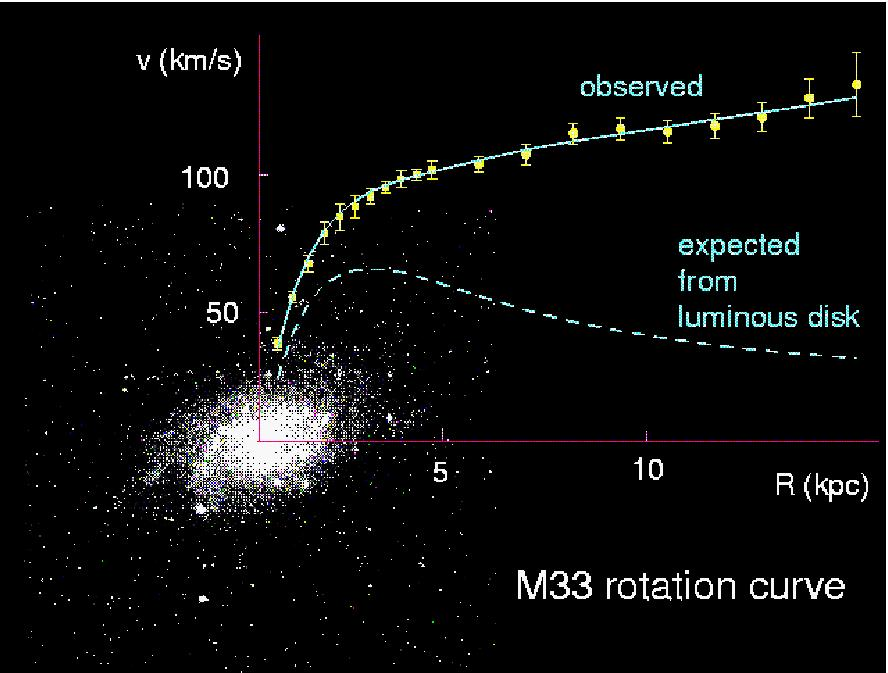
\includegraphics[width=5.5cm,height=4.cm]{rotationCurve.jpg}\\[-0.2cm] 
		\bl{   \fontF E.~Corbelli and P.~Salucci,   {\em Mon.\ Not.\ Roy.\ Astron.\ Soc.\  {\bf 311} 441}  (2000), %\\[-0.3cm]
			\href{https://arxiv.org/abs/astro-ph/9909252}{\fontF  arXiv:astro-ph/9909252}.}  
		\begin{textblock}{0.8}(0.94,1.5)
			\begin{turn}{70}
				{\bf \color{yellow} \Large Hint}
			\end{turn}
		\end{textblock}
		
		\column{0.5\textwidth}
		\vspace{-0.0cm}\centering 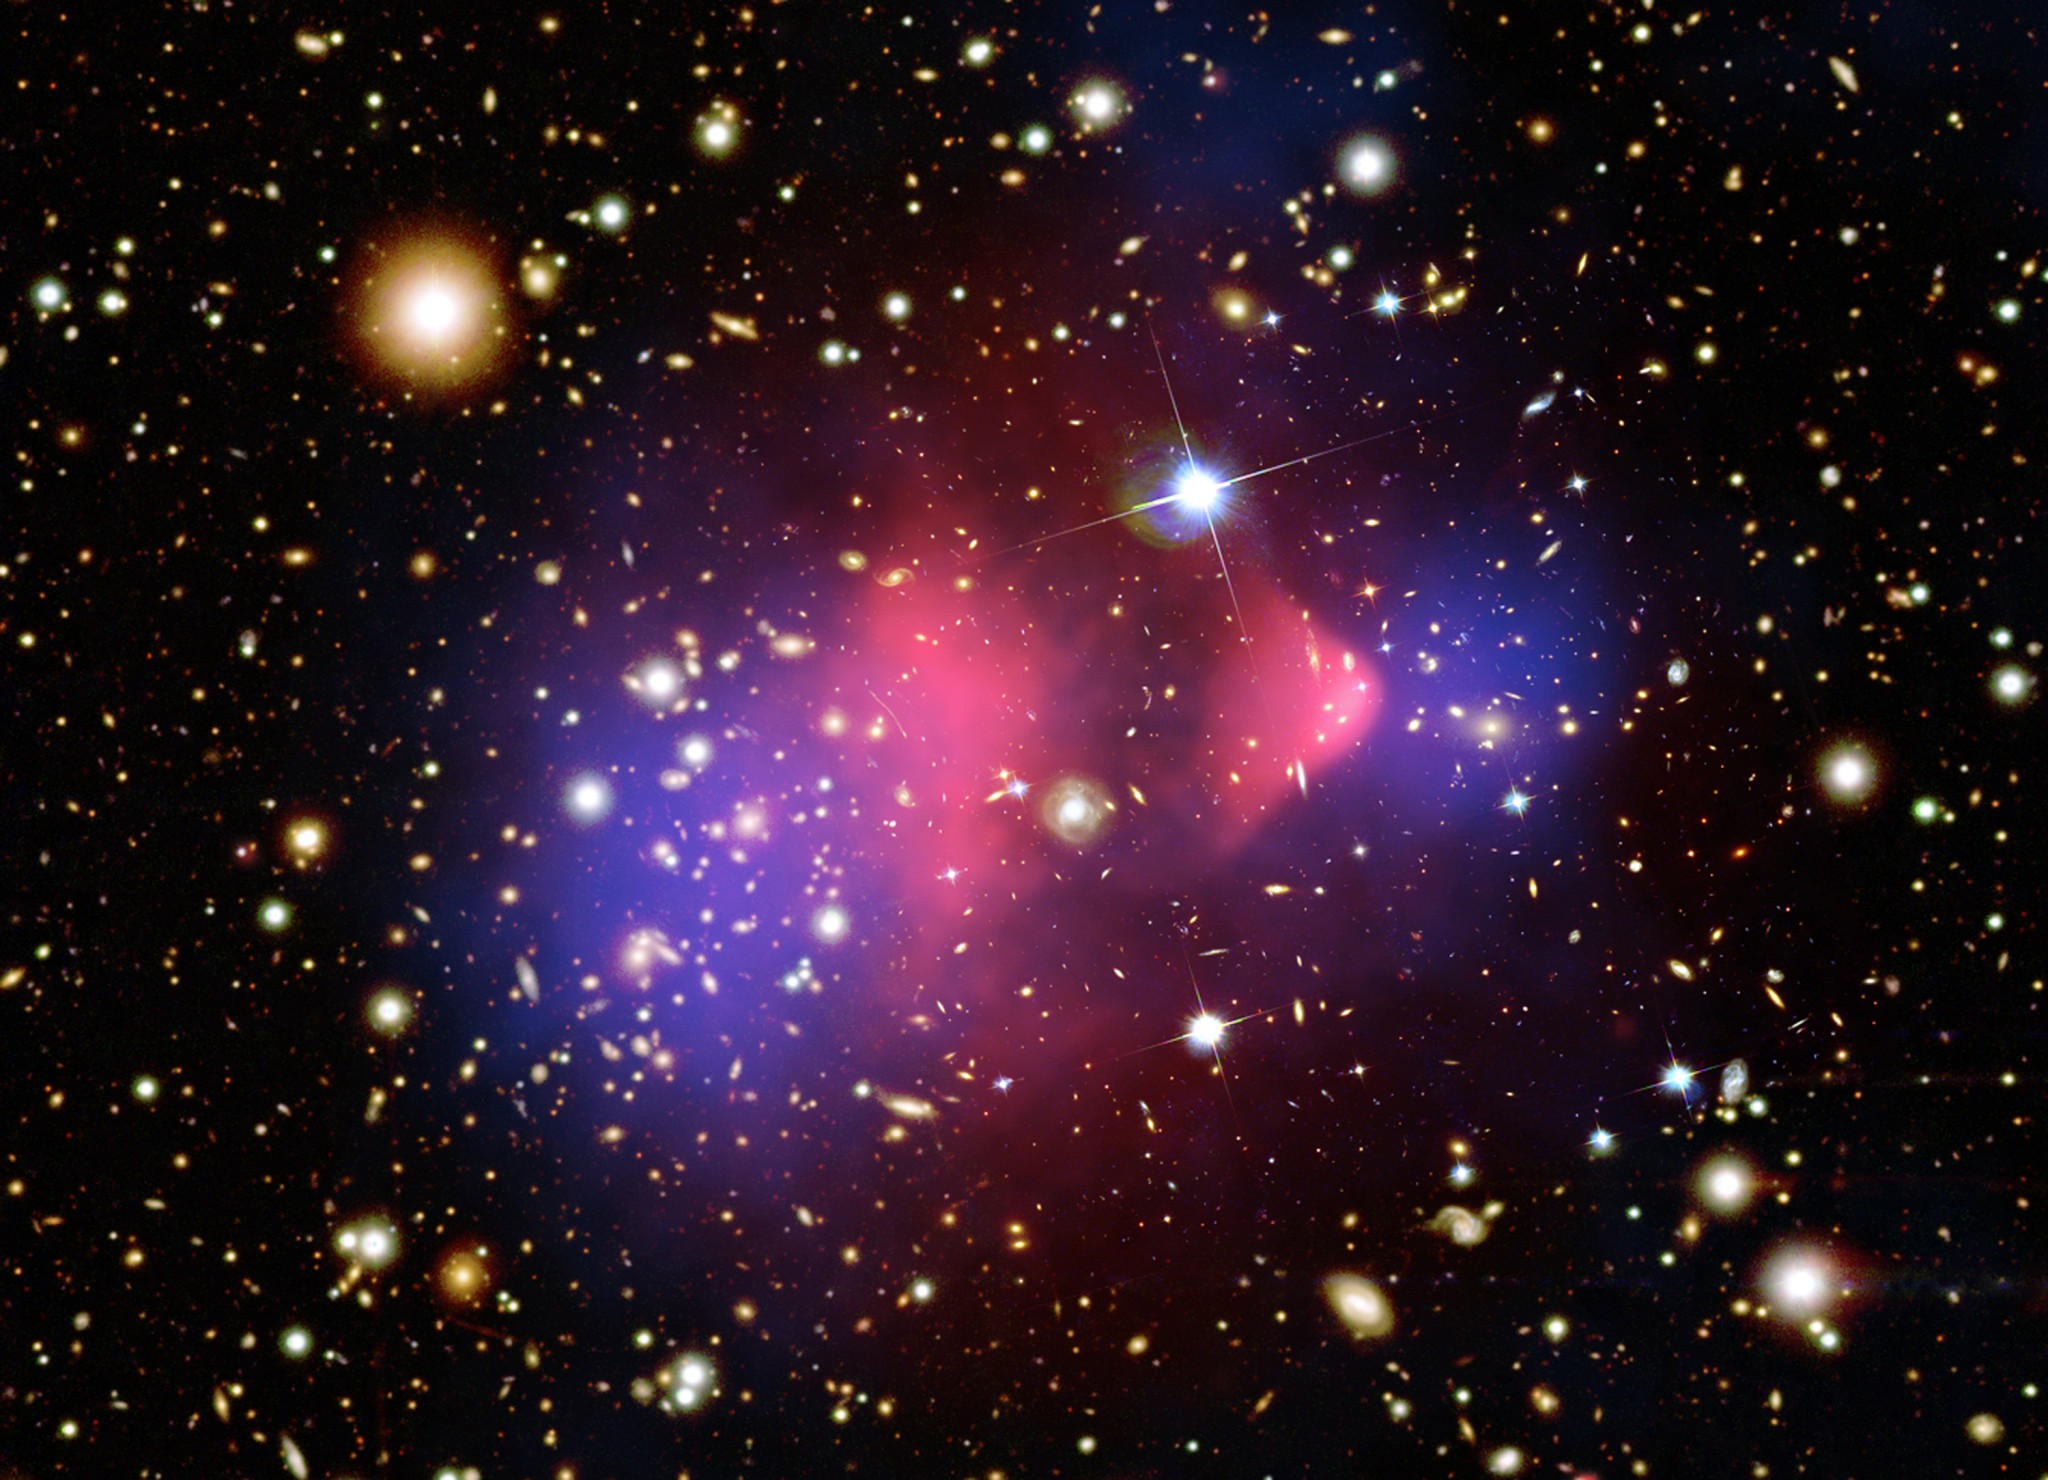
\includegraphics[width=5.5cm,height=4.cm]{BulletCluster.jpg} \\[-0.2cm] 
		\bl{ \fontF   M.~Markevitch, ESA Spec.\ Publ.\  {\bf 604} (2006) 723, \href{https://arxiv.org/abs/astro-ph/0511345}{\fontF  astro-ph/0511345}.%\\[-0.3cm] 
			Clowe, Bradac, {\em  et. al.}  Astrophys.\ J.\  {\bf 648}, L109 (2006),    \href{https://arxiv.org/abs/astro-ph/0608407}{\fontF  astro-ph/0608407}           }
		
	\end{columns}
	\begin{textblock}{0.8}(8.4,1.5)
		\begin{turn}{70}
			{\bf \color{yellow} \Large Evidence}
		\end{turn}
	\end{textblock}
	
	\vspace*{-0.2cm}
	\begin{center}
		
		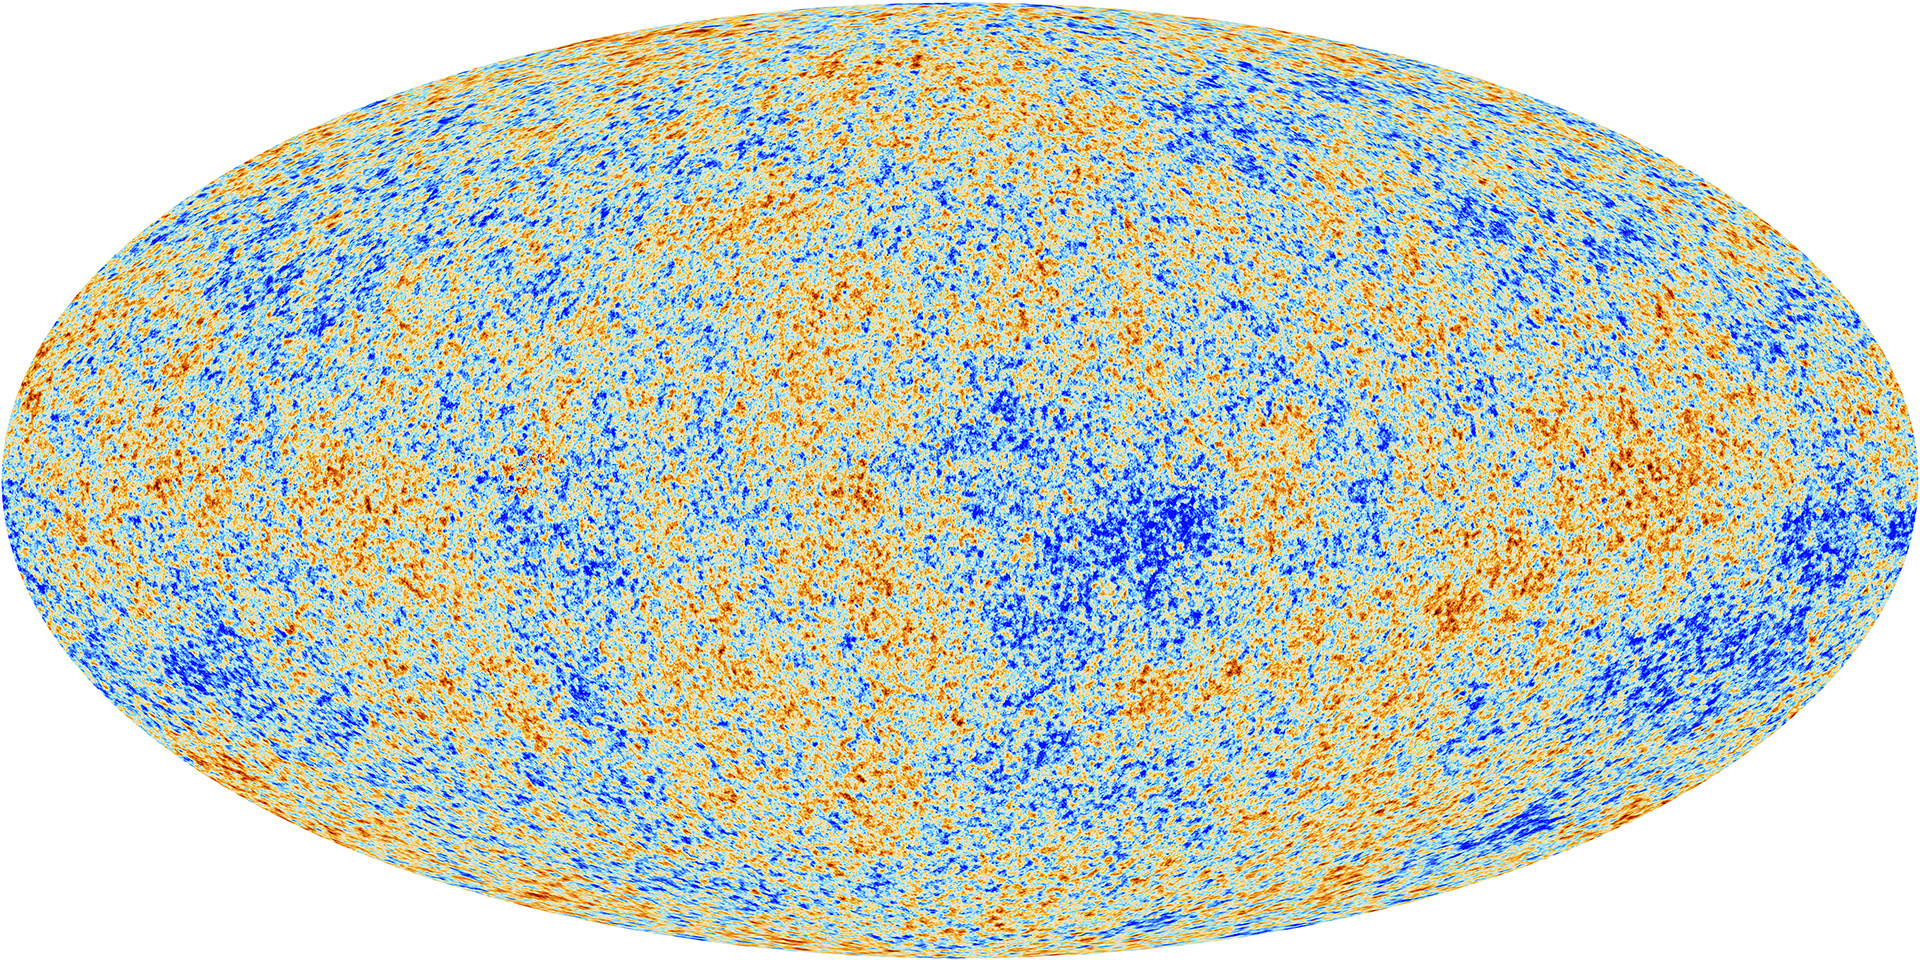
\includegraphics[width=6.cm, height=3.cm]{Planck_CMB.jpg}\\[-0.25cm] 
		\bl{ 
			\fontF  N.~Aghanim {\it et al.} [Planck Collaboration],
			%``Planck 2018 results. VI. Cosmological parameters,''
			\href{https://arxiv.org/abs/1807.06209}{\fontF  arXiv:1807.06209} [astro-ph.CO].
		}
		\begin{textblock}{0.8}(6.2,11.3)
			%				$\Lambda$CDM
			\begin{turn}{0}
				{\color{black}  \Large $\Omega_{\rm DM}h^2 \approx 0.12$}
			\end{turn}
		\end{textblock}
		
	\end{center}	
	
\end{frame}
%%%%%%%%%%%%%%%%%%%%%%%%%%%%%%%%%%%%%%%%%%%%%%%%%%%%%%%%%%%%%%%%%%%%%%%%%%%%%%%%%
\subsection{The dark matter particle}

%\vspace*{-6.5mm}    
%\begin{frame}{\insertsubsectionhead}
%	\hspace*{-11mm}
%	\includegraphics[width=\paperwidth]{You_Know_Nothing.jpg}
%\end{frame} 


%\newgeometry{margin=0pt}
%%%%%%%%%%%%%%%%%%%%%%%%%%%%%%%%%%%%%%%%%%%%%%%%%%%%%%%%%%%%%%%%%%%%%%%%%
\begin{frame}{\insertsubsectionhead}
	\begin{center}
%		\begin{otherlanguage}{greek}
%			<<Έν οἶδα, ὅτι οὐδὲν οἶδα.>>\\
%		\end{otherlanguage}		
		``I know one thing,  that I know nothing.''
		\flushright --Socrates %\pause
	\end{center}
	
	%	Properties:\pause
	\begin{itemize}
		\item Gravitational interactions.
		\item Mostly electrically neutral.
		\item Stable or very slow decay rate. 
		\item Non-Baryonic.
		\item Cold/Warm and non-relativistic today.
	\end{itemize}
	
\end{frame}
%%%%%%%%%%%%%%%%%%%%%%%%%%%%%%%%%%%%%%%%%%%%%%%%%%%%%%%%%%%%%%%%%%%%%%%%%

%%%%%%%%%%%%%%%%%%%%%%%%%%%%%%%%%%%%%%%%%%%%%%%%%%%%%%%%%%%%%%%%%%%%%%%%%
\subsection{The axion (like) particle}
\begin{frame}{\insertsubsectionhead}
	%
	Notably, the original axion was originally introduced in order to solve the {\em strong-CP problem} of the SM.
	Axion-like-particles (ALPs) arise in a number of new physics models, beyond the SM.  \\[0.5cm]
	
	Axions and ALPs generally:
	%
	\begin{itemize}
		\item Have suppressed interactions with photons.
		\item Are (mostly) stable. 
		\item Were non-relativistic around the epoch of structure formation. 
		\item Non-baryonic (by definition), and of-course interact gravitationally.\pause\\[1cm]
	\end{itemize}
	
	\begin{center}
		{\bf \em Maybe DM has axionic nature!}	
	\end{center}
	
\end{frame}
%%%%%%%%%%%%%%%%%%%%%%%%%%%%%%%%%%%%%%%%%%%%%%%%%%%%%%%%%%%%%%%%%%%%%%%%%


%%%%%%%%%%%%%%%%%%%%%%%%%%%%%%%%%%%%%%%%%%%%%%%%%%%%%%%%%%%%%%%%%%%%%%%%%
\section{Calculating the Relic Abundance}
\subsection{The axion EOM}
\begin{frame}{\insertsubsectionhead}
	%
	Axions and ALPs follow a similar equation of motion (EOM):
	\begin{equation*}
		\lrb{\dfrac{d^2}{d t^2} + 3 H(t) \ \dfrac{d}{d t} } \theta(t) + \maT^2(t) \ \sin \theta(t) = 0 \; ,
	\end{equation*}	
	%
	where $\theta= A \, \fa$, with $A$ the axion filed, and $\fa$ some energy scale that characterises the potential (Peccei-Quinn breaking scale).
	
	
\end{frame}
%%%%%%%%%%%%%%%%%%%%%%%%%%%%%%%%%%%%%%%%%%%%%%%%%%%%%%%%%%%%%%%%%%%%%%%%%

%%%%%%%%%%%%%%%%%%%%%%%%%%%%%%%%%%%%%%%%%%%%%%%%%%%%%%%%%%%%%%%%%%%%%%%%%
\subsection{How hard can it be?}
\begin{frame}{\insertsubsectionhead}
	%
	\begin{center}
		\textbf{Hard} (in general).\\[1cm]
	\end{center}	
	
	The classical analogue is the dumped pendulum with both frequency (length) and friction being time-dependent:
	%
	\begin{itemize}
		\item There is no closed form solution.
		\item There are no constants of motion (wait a minute...).
		\item No package/library/program available!\pause\\[1cm]
	\end{itemize}
	
	\begin{center}
		{\sl \mimes simulates the evolution of the axion/ALP, for (virtually) any cosmological scenario and axion/ALP (thermal) mass.}
	\end{center}		
\end{frame}
%%%%%%%%%%%%%%%%%%%%%%%%%%%%%%%%%%%%%%%%%%%%%%%%%%%%%%%%%%%%%%%%%%%%%%%%%

%%%%%%%%%%%%%%%%%%%%%%%%%%%%%%%%%%%%%%%%%%%%%%%%%%%%%%%%%%%%%%%%%%%%%%%%%
\subsection{Initial conditions}
\begin{frame}{\insertsubsectionhead}
	%
	Some time at the very early Universe, $\maT \ll H(T)$,~\footnote{\fontF This is an assumption that \mimes has to make for the sake of generality.} with
	\begin{equation*}
		\ddot{\theta}  + 3H \ \dot{\theta} \approx 0 \;.
	\end{equation*}	
	%
	The solution is 
	$$
	\theta = \thetai + C \dint_{0}^t d t' \ \lrb{ \dfrac{a(t'=0)}{a(t')} }^3 \;.
	$$
	%this is true especially in the case where the PQ symmetry breakes before inflation.
	So, $\dot{\theta} \sim a^{-3}$. Since we are interested in $\theta$ at much later times (once the potential becomes relevant), $\dot{\theta} \approx 0$.%~\footnote{\fontF Standard misalignment mechanism. For the kinetic one see
%		
%		\bl{\fontF R.~T.~Co, L.~J.~Hall and K.~Harigaya,
%			\href{https://doi.org/10.1103/PhysRevLett.124.251802}{Phys. Rev. Lett. \textbf{124} (2020) no.25, 251802}
%			\href{https://arxiv.org/abs/1910.14152}{[arXiv:1910.14152 [hep-ph]]}},
%		%
%		\bl{\fontF  C.~F.~Chang and Y.~Cui,
%			\href{https://doi.org/10.1103/PhysRevD.102.015003}{Phys. Rev. D \textbf{102} (2020) no.1, 015003}
%			\href{https://arxiv.org/abs/1911.11885}{[arXiv:1911.11885 [hep-ph]]}}, or 
%		% 
%		\bl{\fontF  B.~Barman, N.~Bernal, N.~Ramberg and L.~Visinelli,
%			\href{https://arxiv.org/abs/2111.03677}{[arXiv:2111.03677 [hep-ph]]} }.	
%	}
	%
	Therefore, we can begin integration at some point with $3H \gg \maT$, and set $\theta(t=\ti) = \thetai$ and $\dot \theta(t=\ti) = 0$. 
	
\end{frame}
%%%%%%%%%%%%%%%%%%%%%%%%%%%%%%%%%%%%%%%%%%%%%%%%%%%%%%%%%%%%%%%%%%%%%%%%%
\subsection{(Bad) Approximations}
\begin{frame}{\insertsubsectionhead}

%	\begin{center}
%		``He who thinks great thoughts, often makes great errors.''
%		\flushright --Martin Heidegger %\pause
%	\end{center}

	\begin{center}
		``If a man knows not which port he sails, no wind is favourable.''
		\flushright --Seneca %\pause
	\end{center}


%	Once we agree on the initial conditions, we move to the next important things:\pause
%		
	%\begin{equation*}
	%	\ddot \theta + \underbrace{  \bl{ 3\overbrace{H(t) }^{\text{Slow}}  } \ \dot \theta + \bl{ \overbrace{\maT^2(t)}^{\text{Slow}}  }}_{\maT > 3 H} \ \rd{\underbrace{ \sin \theta(t) }_{\theta \ll 1}  } = 0 \; ,
	%\end{equation*}	
	%
	\begin{itemize}
		\item Assume $\theta \ll 1$, and linearise the EOM. {\sl Not general.}
		\item Assume that at $\maT(\Tosc) \approx 3H(\Tosc)$ we have $\dot\theta(\Tosc)=0$. {\sl Not very precise.}
		\item Assume that $\thetaosc \approx \thetai$. {\sl Generally quite bad.}\pause
	\end{itemize}
	
	These result in ``WKB''-approximate solution
	%
	\begin{equation*}\vspace*{-0.2cm}
		\theta(t) \approx \thetai \lrb{\dfrac{3}{4}}^{1/4} \sqrt{ \dfrac{ \maT(\Tosc) }{\maT(T)} } \lrb{\dfrac{a}{\aosc}}^{-3/2} \  \cos\lrb{ \int_{\tosc}^t d t^\prime  \ \maT(t^\prime)}   \;,
	\end{equation*}
	%
	which gives us:
	%
	\begin{equation*}\vspace*{-0.2cm}		
		\rho_{a,0} = \gamma^{-1}  \dfrac{s_0}{s_{\rm osc}} \  \dfrac{1 }{2}  \ \fa^2 \ \ma \ \maT_{,{\rm osc}} \ \thetai^2    \;,
	\end{equation*}
	%
	where $\gamma$ the amount of entropy injection between $\Tosc$ and today.%~\footnote{\fontF Defined from $s(T_0) = \gamma \ \aosc^3 \ s_{\rm osc}$.}
\end{frame}
%%%%%%%%%%%%%%%%%%%%%%%%%%%%%%%%%%%%%%%%%%%%%%%%%%%%%%%%%%%%%%%%%%%%%%%%%
\subsection{Need for speed, accuracy, and automation}
\begin{frame}{\insertsubsectionhead}
	%
	Life before \mimes: \\[1cm]\pause
	%
	\begin{itemize}
		\item No available tool that can help us reproduce published results obtained by numerical integration. \emph{Reproducing results means reproducing effort}.\pause
		\item The approximations can be tested against numerical results in a case-by-case basis. \emph{No measure of accuracy}.\pause%There is no way to tell if they will work in new models and cosmological scenarios.
		\item Simply checking if an ALP model is compatible with a cosmological scenario is \emph{slow} or \emph{inaccurate}. 
	\end{itemize}
	
	
	
\end{frame}




%%%%%%%%%%%%%%%%%%%%%%%%%%%%%%%%%%%%%%%%%%%%%%%%%%%%%%%%%%%%%%%%%%%%%%%%%
\section{\mimes}
\subsection{\mimes: Why?}
\begin{frame}{\insertsubsectionhead}
	We need accurate code that solves the EOM, but most importantly we need {\sl reproducible} results! \\[0.2cm]
	
	\mimes is:
	% 
	\begin{itemize}
		\item \mimes is a \CPP header-only library that contains various templated classes. 
%		
		\item \mimes comes with a \PY interface.
%
		\item Is {\sl easy} to use; anyone can run it and see if their model can work or check against the literature.
%
		\item Is reasonably fast; less than $0.05 \; s$ for the scenarios tested.
%
		\item Provides full access to results and their errors, which can help determine if the results are accurate.
%
		\item Asks the user to decide when to start, stop, and when adiabaticity is reached.
	\end{itemize}
	
\end{frame}
%%%%%%%%%%%%%%%%%%%%%%%%%%%%%%%%%%%%%%%%%%%%%%%%%%%%%%%%%%%%%%%%%%%%%%%%%

\subsection{\mimes: Under the hood}
\begin{frame}{\insertsubsectionhead}
	%
	\begin{center}
	%		\begin{otherlanguage}{greek}
	%			<<Έν οἶδα, ὅτι οὐδὲν οἶδα.>>\\
	%		\end{otherlanguage}		
		``It is the empty space which makes a bowl useful.''
		\flushright --Laozi %\pause
	\end{center}
	%
	\mimes is built as minimally as possible:
	\\[0.3cm] 
	%
	\begin{itemize}
		\item \mimes relies on \cppin{NaBBODES}~\footnote{\fontF \href{https://github.com/dkaramit/NaBBODES}{https://github.com/dkaramit/NaBBODES}.} \cppin{SimpleSplines}~\footnote{\fontF \href{https://github.com/dkaramit/SimpleSplines}{https://github.com/dkaramit/SimpleSplines}.}.
		\item You only need to have the standard \CPP library.
		\item The two libraries are developed by myself, so their integration with \mimes is seamless.
		\item There is always going to be a compatible version of these libraries that works with \mimes.\\[0.3cm]
	\end{itemize}	
		
\end{frame}

\subsection{\mimes: the \emph{solver} part}
\begin{frame}{\insertsubsectionhead}
	
\end{frame}
%%%%%%%%%%%%%%%%%%%%%%%%%%%%%%%%%%%%%%%%%%%%%%%%%%%%%%%%%%%%%%%%%%%%%%%%%
%\subsection{\mimes: Notation}
%\begin{frame}{\insertsubsectionhead}
%	%
%	\vspace{-0.2cm}
%	
%	``Time'' in \mimes:
%	 %
%	\begin{equation*}\vspace{-0.2cm}
%		u \equiv \log \lrb{a/\ai}\;.
%	\end{equation*} 
%	%
%	~\footnote{\fontF With $\ai$ some initial value of the scale factor}
%	%
%	The EOM is transformed to
%	%
%	\begin{eqnarray*}\vspace*{-0.5cm}
%		& \dfrac{d  \zeta}{du} + \lrsb{\dfrac{1}{2} \dfrac{d \log H^2}{du} + 3 } \zeta + \ \lrb{\dfrac{\maT}{H}}^2 \ \sin \theta
%		=0 \;. \\[-0.2cm]
%		&\dfrac{d \theta}{d u} - \zeta=0 \;.
%	\end{eqnarray*}\\[-0.2cm]
%	%
%	The initial conditions are $\zeta(0)=0$ and $\theta(0)=\thetai$.\\[1cm]\pause
%	
%	\begin{center}
%		{\em This is the same notation as in the code} $\Rightarrow$ {\em You can change it easily.}
%	\end{center}
%	
%	
%\end{frame}

%%%%%%%%%%%%%%%%%%%%%%%%%%%%%%%%%%%%%%%%%%%%%%%%%%%%%%%%%%%%%%%%%%%%%%%%%
%\subsection{Ingredients for numerical integration: Adiabatic invariant}
%\begin{frame}{\insertsubsectionhead}
%	%
%	If a system exhibits closed orbits, the quantity
%	%
%	\begin{equation*}
%		J \equiv C \ \oint p \ d \theta \;,
%	\end{equation*}
%	%
%	is the adiabatic invariant. In this case, it becomes
%	%
%	\begin{equation*}
%		J = a^3 \ \maT \ \thetamax^2  \, f(\thetamax)  \;,
%	\end{equation*}
%	%
%	with 
%	\begin{equation*}
%		f(\thetamax) =\dfrac{ 2 \sqrt{2}}{\pi \thetamax^2 } \dint_{- \thetamax}^{\thetamax} d \theta \sqrt{ \cos \theta - \cos \thetamax } \;,
%	\end{equation*}
%	%
%	the so-called anharmonic factor.\pause
%	
%	\textbf{Important}: $\thetamax$ is the peak of the oscillation. So, $J$ can be used to determine how $\thetamax$ changes with time. By definition, at $\theta=\thetamax$, $p \sim \dot \theta = 0$.
%	This means that we can find $\rho_{a,0}$ on the peak of today's $\theta$, as
%	%
%	\begin{equation*}
%		\rho_{a,0} = \gamma^{-1} \ \dfrac{s_0}{s_*} \ \ma \ \maT_{,*} \ \dfrac{1}{2} \ \fa^2 \ \thetamax_{,*}^2 \;  \ f(\thetamax_{,*}) \;,
%	\end{equation*}
%	%
%	where $T_{*}$ the temperature at which adiabaticity was reached, and $\gamma$ the entropy injection between $T_*$ and today (\ie $s_0 = \gamma a_*^3 s_*$). 	  
%\end{frame}
%
%
%%%%%%%%%%%%%%%%%%%%%%%%%%%%%%%%%%%%%%%%%%%%%%%%%%%%%%%%%%%%%%%%%%%%%%%%%%
%\subsection{Ingredients for numerical integration: Integration limits}
%\begin{frame}{\insertsubsectionhead}
%	%
%	The starting condition should be: 
%	\begin{itemize}
%		\item At a point with $\dot \theta=0$.
%		\item At some $\Ti$ with $3H(\Ti)/\maT(\Ti) \gg 1$.
%		\item Such that the evolution of $\theta$ is the same for any other starting point with $T>\Ti$.
%		\item {\em User defined, so that we can change it the cosmology.}
%	\end{itemize}
%	
%	The stopping condition should be:
%	\begin{itemize}
%		\item At a point, $T = T_*$, with $\Delta J/J \leq \epsilon \ll 1$.
%		\item Such that the evolution of $\theta$ is the same for any other end point with $T<T_*$.
%		\item {\em User defined, so that we can change it the cosmology.}
%	\end{itemize}
%	
%	
%	
%	
%\end{frame}
%%%%%%%%%%%%%%%%%%%%%%%%%%%%%%%%%%%%%%%%%%%%%%%%%%%%%%%%%%%%%%%%%%%%%%%%%

%%%%%%%%%%%%%%%%%%%%%%%%%%%%%%%%%%%%%%%%%%%%%%%%%%%%%%%%%%%%%%%%%%%%%%%%%

\section{Using \mimes}

\subsection{How to get \mimes}
\begin{frame}[fragile]{\insertsubsectionhead}
	There are several ways you can get a stable version of \mimes:
	\begin{enumerate}
		%
		\item \cppin{git clone -b stable https://github.com/dkaramit/MiMeS.git}. This is the preferred way, as it is guaranteed to be the latest stable version.
		%
		\item Go to \href{https://mimes.hepforge.org/downloads}{mimes.hepforge.org/downloads}, and download it. 
		%
		\item Go to \href{https://github.com/dkaramit/MiMeS/releases}{github.com/dkaramit/MiMeS/releases}, and download a released version.    
	\end{enumerate}
	
	
	You can get the most up-to-date code -- not always the most stable one -- including the latest version of {\tt NaBBODES} and {\tt SimpleSplines}, by running
	%
	\begin{lstlisting}
	git clone https://github.com/dkaramit/MiMeS.git
	cd MiMeS
	git submodule init
	git submodule update --remote
	\end{lstlisting}
	
\end{frame}

\subsection{Configure (and make)}
\begin{frame}[fragile]{\insertsubsectionhead}
	There is no need to install anything if you are going to use \mimes in a \CPP program. The only thing you {\em must} do is run 
	\begin{bash}
		bash configure.sh
	\end{bash}
	%	
	Alter that, you can include the header file \cppin{MiMeS/MiMeS.hpp}, and you are good to go.
	
	However, you can also run 
	%
	\begin{itemize}
		\item \cppin{make lib}, in order to produce the (shared) libraries. This is needed in order to run the \PY interface. 
		\item \cppin{make examples}, in order to compile the examples in \cppin{MiMeS/UserSpace/Cpp}.
		\item \cppin{make exec}, in order to produce some test executables  (in \cppin{MiMeS/exec}). You just need to run then in order to see if you get any segfaults.
	\end{itemize}
\end{frame}


\subsection{Classes}
\begin{frame}[fragile]{\insertsubsectionhead}
	There are three classes useful to the user.~\footnote{\fontF There are various arguments that need to be passed to the constructors, and the are all listed and explained in the Appendix of the documentation.}\pause
	%
	\begin{itemize}
		\item \cppin{mimes::Cosmo<LD>}: interpolation of relativistic degrees of freedom of the plasma. By default it uses the EOS2020~\footnote{\fontF 
			\bl{K.~Saikawa and S.~Shirai,
				\href{https://doi.org/10.1088/1475-7516/2020/08/011}{JCAP \textbf{08} (2020), 011}
				\href{https://arxiv.org/abs/2005.03544}{[arXiv:2005.03544 [hep-ph]]}.}
		} data. The user can choose another file easily.
		%
		\pause
		%
		\item \cppin{mimes::AxionMass<LD>}: definition of axion/ALP mass as a function of the temperature and $\fa$. \mimes is shipped with data from Lattice calculation~\footnote{\fontF \bl{
				S.~Borsanyi, Z.~Fodor, J.~Guenther, K.~H.~Kampert, S.~D.~Katz, T.~Kawanai, T.~G.~Kovacs, S.~W.~Mages, A.~Pasztor and F.~Pittler, \textit{et al.}
				\href{https://doi.org/10.1038/nature20115}{Nature \textbf{539} (2016) no.7627, 69-71}
				\href{https://arxiv.org/abs/1606.07494}{[arXiv:1606.07494 [hep-lat]]}.}} of the QCD axion mass.
		%
		\pause
		%	
		\item \cppin{mimes::Axion<LD,Solver,Method>}: This is responsible for actually solving the EOM.
	\end{itemize}
	
	
\end{frame}




\subsection{Template arguments}
\begin{frame}[fragile]{\insertsubsectionhead}
	%
	You need to choose what numeric type to use. This is done by the template argument \cppin{LD} which should be \cppin{double} (fast) or \cppin{long double} (accurate).~\footnote{\fontF You could choose \cppin{float}, but we live in 2021.}\\[0.5cm]
	
	
	You also need to tell \mimes which integration strategy to use. This is done by choosing template arguments:
	%
	\begin{itemize}
		\item \cppin{Solver} can be set to \cppin{1} for Rosenbrock (semi-implicit Runge-Kutta). 
		The \cppin{Method} argument in this case can be:\\[-0.0cm]
		\begin{itemize}
			\item \cppin{RODASPR2<LD>} (4th order).
			\item \cppin{ROS34PW2<LD>} (3rd order).
			\item \cppin{ROS3W<LD>} (2rd order, {\em very} bad).
		\end{itemize}
		\item \cppin{Solver} can be set to \cppin{2} for explicit RK.
		The \cppin{Method} argument can be:\\[-0.0cm]
		\begin{itemize}
			\item \cppin{DormandPrince<LD>} (7th order)
			\item \cppin{CashKarpRK45<LD>} (5th order, {\em very} bad).
			\item \cppin{RK45<LD>} (5th order, {\em very} bad).
		\end{itemize}	
	\end{itemize}
\end{frame}

\subsection{\mimes from \PY}
\begin{frame}[fragile]{\insertsubsectionhead}
	In order to call the \PY interface of \mimes, we need to first call \cppin{make lib} in the root directory of \mimes.\\[0.2cm]
	
	Before that, we can take some time to decide what the template arguments and compilation  options should be. In the 
	file \cppin{MiMeS/Definitions.mk}, you can change the variables:
	%
	\begin{itemize}
		\item \cppin{LONGpy=long} will compile the library with \cppin{long double} numeric types. \cppin{LONGpy=} will compile the library with \cppin{double} numeric types.
		\item \cppin{SOLVER} and \cppin{METHOD}, as in the template arguments.
	\end{itemize}
	
	Also, in the same file, you can change compilation options:
	%
	\begin{itemize}
		\item Compiler:
		\begin{itemize}
			\item \cppin{CC=g++} in order to use the \cppin{GNU} \CPP compiler.
			\item \cppin{CC=clang -lstdc++} in order to use the \cppin{clang} \CPP compiler.
		\end{itemize}
		\item Optimization level:
		\begin{itemize}
			\item \cppin{OPT=O0}: No optimization. 
			\item \cppin{O=O1}, \cppin{O2}, or \cppin{O3}: all these perform mostly the same (read the compiler documentation for more information on the optimization).
			\item \cppin{OPT=Ofast}: full optimization (fast, but dangerous). 
		\end{itemize}
	\end{itemize}
\end{frame}

\subsection{Assumptions}
\begin{frame}[fragile]{\insertsubsectionhead}
	
	\mimes is designed to make as few assumptions as possible. However, it still assumes that:\pause
	%
	\begin{enumerate}
		\item $H/\maT$ increases monotonically with the temperature.\pause
		\item $\zeta(0)=0$. This will be changed in the future.\pause
		\item The energy density of the axion/ALP is always subdominant.\pause
		\item Only the EOM determines the energy density (no annihilations, no strings, etc.).
	\end{enumerate}	
\end{frame}


\subsection{What \mimes expects from you}
\begin{frame}[fragile]{\insertsubsectionhead}
	Apart from $\thetai$ and $\fa$, keep in mind that \mimes needs:\pause
	%
	\begin{enumerate}
		\item The mass of the axion/ALP. A data file or an actual function.\pause
		\item Data file with $\log a/a_i$ ($a_i$ is some arbitrary value; \mimes rescales it appropriately), $T$, and $\log H$ of the underlying cosmology.\pause
		\item Value for $3H/\maT \gg 1$, which defines the point where integration begins.\pause
		\item Relative difference of $J$ between a given number of peaks at which we consider adiabaticity to have been reached.\pause
		\item Other input, such as the temperature at which integration exits.
	\end{enumerate}
\end{frame}



\section{Examples}

\subsection{\PY}
\begin{frame}[fragile]{\insertsubsectionhead}
	Define everything and solve in just a few lines of code!\\[-0.15cm]
	\lstset{language = python}
	\lstinputlisting[basicstyle=\fontF]{example.py}
	
\end{frame}
\subsection{\CPP}
\begin{frame}[fragile]{\insertsubsectionhead}
	
	{\em Notice}: \CPP and \PY are quite similar!\\[-0.15cm]
	\lstset{language = c++}
	\lstinputlisting[basicstyle=\fontF]{example.cpp}
\end{frame}

\section{Outlook}

%\subsection{Summing up}
%\subsection{Future}
\begin{frame}[fragile]{\insertsectionhead}
	\begin{center}
		\bf{What we saw:}
	\end{center}
	%
	\begin{itemize}
		\item \mimes solves the axion/ALP EOM. 
		\item \mimes treats both the mass and the underlying cosmology as user inputs.
		\item \mimes allows the user to change a number of other things, from the plasma RDOFs to the convergence conditions.\\[0.5cm] 
	\end{itemize}
	
	\begin{center}
		\bf{\mimes may be amended in the future because:} 
	\end{center}
	%
	\begin{itemize}
		\item \mimes should allow the user to consider different initial value of $\zeta$; the ''kinematic'' \mimes might come soon.
		\item \mimes should be able to handle non-vanishing \rhs; \ie solve the ''driven'' dumped time-dependent pendulum.
		%		\item Would be nice if \mimes could handle case of freeze-out/in.
		\item \mimes should be able to compare against searches on the fly. 
	\end{itemize}
	
\end{frame}


\setbeamercolor{structure}{fg=black!80!red}
\setbeamercolor{section in head/foot}{fg=white, bg=red}
\setbeamertemplate{footline}{
	%\begin{beamercolorbox}[wd=1\textwidth,ht=2.25ex,dp=1ex,right]{section in head/foot}%
	%\insertsubsectionhead 
	%\insertframenumber/\inserttotalframenumber
	%\end{beamercolorbox}
}
\setbeamertemplate{background canvas}{%
	
\begin{tikzpicture}[remember picture,overlay]
	\shade[left color=red!90!black, right color=black!80!red]
	([shift={(0.0cm,-0.0cm)}]current page.north west)
	rectangle
	([shift={(-0.0cm,0.0cm)}]current page.south east);
	\end{tikzpicture}%     
}
%\setbeamercolor{background canvas}{bg=red}
\begin{frame}[noframenumbering]
	
	\begin{center}
		{\color{yellow} \Huge Thank you!}\\[0.5cm]
		
		{\color{yellow}Breakdown of \mimes}:\\
		{\fontsize{10}{1} \selectfont \color{white} \verbatiminput{cloc.txt}}
	\end{center}
	
	\begin{center}
		\href{https://github.com/dkaramit/MiMeS}{ 
\includegraphics[width=2.5cm]{GitHub.png} }
		\hfill
		\href{https://mimes.hepforge.org}{
\includegraphics[width=2.5cm]{hepforge.png}}
	\end{center}
\end{frame}




\setbeamertemplate{background canvas}{%
	
\begin{tikzpicture}[remember picture,overlay]
	\shade[left color=black!90!red, right color=red!80!black]
	([shift={(0.0cm,-0.0cm)}]current page.north west)
	rectangle
	([shift={(-0.0cm,0.0cm)}]current page.south east);
	\end{tikzpicture}%     
}

%%Put equations for Back-up. 
\begin{frame}[noframenumbering]
	%	
	\begin{center}
		{\color{yellow} \Huge Backup \\ {\tiny (equations, derivations, tables)}}
	\end{center}
	%	
\end{frame}
%
\setbeamertemplate{background canvas}{}
\setbeamercolor{background canvas}{bg=white}

\begin{frame}{WKB -- I}
	\begin{equation*}
		\lrb{\dfrac{d^2}{d t^2} + 3 H(t) \ \dfrac{d}{d t} + \maT^2(t) } \theta(t) = 0 \; .
	\end{equation*}
	%
	Reparametrize by introducing
	% 
	\begin{equation*}
		\theta_{\rm trial} = \exp\lrsb{ i \dint d t \ \lrBigb{\psi(t) +3/2 \ i \ H(t)} } \;.
	\end{equation*}
	%
	The Eome, then becomes just
	%
	\begin{equation*}
		\psi^2 = \Omega^2 + i \ \dot \psi \; ,
	\end{equation*}
	%
	with $\Omega^2 = \maT^2 - \dfrac{9}{4} H^2 -  \dfrac{3}{2} \dot H $.
	%
	The solution takes the form $\psi = \pm \sqrt{\Omega^2 + i \dot \psi}$. However, for $\dot \psi \ll \Omega^2$ and $\dot \Omega \ll \Omega^2$, it can be approximated as
	%
	\begin{equation*}
		\psi \approx \pm \Omega + \dfrac{i}{2} \dfrac{d \log \Omega}{d t} \;.
	\end{equation*}
\end{frame}

\begin{frame}{WKB -- II}
	So, after applying the initial conditions, the EOM is solved by
	%
	\begin{equation*}
		\theta(t) \approx \thetai \sqrt{ \dfrac{ \Omegai }{\Omega (t)} } \lrb{\dfrac{a}{\ai}}^{-3/2} \  \cos\lrb{ \int_{\ti}^t d t^\prime  \ \Omega(t^\prime)}   \;.
	\end{equation*}
	
	Taking  $\ti = \tosc$ (\ie $\dot \theta(\tosc) = 0$, which is not generally good), have
	%
	\begin{equation*}
		\theta(t) \approx \thetaosc \lrb{\dfrac{3}{4}}^{1/4} \sqrt{ \dfrac{ \maT|_{t=\tosc} }{\maT  (t)} } \lrb{\dfrac{a}{\aosc}}^{-3/2} \  \cos\lrb{ \int_{\tosc}^t d t^\prime  \ \maT(t^\prime)}   \;,
	\end{equation*}
	%
	where $\thetaosc = \theta|_{t=\tosc}$. This equation is further simplified if we assume that $\thetaosc \approx \thetai$ (again not really good), \ie
	%
	\begin{equation*}
		\theta(t) \approx \thetai \lrb{\dfrac{3}{4}}^{1/4} \sqrt{ \dfrac{ \maT|_{t=\tosc} }{\maT  (t)} } \lrb{\dfrac{a}{\aosc}}^{-3/2} \  \cos\lrb{ \int_{\tosc}^t d t^\prime  \ \maT(t^\prime)}   \;.
	\end{equation*}
	
	
\end{frame}

\begin{frame}{Adiabatic invariant -- I}
	%	
	Given a system with Hamiltonian $\mathcal{H}(\theta,p;t)$, the equations of motion are 
	%
	\begin{equation*}
		\dot p = - \dfrac{\partial \mathcal{H}}{\partial \theta} \;, \;\; 
		\dot \theta =  \dfrac{\partial \mathcal{H}}{\partial p} \;.
	\end{equation*}
	%
	Also,
	%
	\begin{equation*}
		d \Ham = \dot \theta \ d p - \dot p \ d \theta + \dfrac{\partial \Ham}{\partial t} \ d t \;.  
	\end{equation*}
	
	
	If this system exhibits closed orbits (\eg if it oscillates), we define 
	%
	\begin{equation*}
		J \equiv C \ \oint p \ d \theta \;,
	\end{equation*}
	%
	where the integral is over a closed path (\eg a period, $T$), and $C$ indicates that $J$ can always be rescaled with a constant. If the Hamiltonian varies slowly during a cycle,
	%
	\[
	\dfrac{d J}{d t} = C \ \oint \lrBigb{\dot p \ d \theta + p \ d \dot \theta} = C \ \dint_{t}^{t+T}  \dfrac{\partial \Ham}{\partial t^\prime} \ d t^\prime \approx T \ \dfrac{\partial \Ham(t^{\prime})}{\partial t^{\prime}}\Big|_{t^{\prime}=t} \approx 0 
	\;. 
	\]
	%
	So, $J$ is an adiabatic invariant!
	
\end{frame}

\begin{frame}{Adiabatic invariant -- II}
	%
	The Hamiltonian that results in the EOM
	%
	\begin{equation*}
		\Ham = \dfrac{1}{2} \dfrac{p^2}{\fa^2 \ a^3} + V(\theta) \ a^3\;,
	\end{equation*}
	%
	with 
	%
	\begin{eqnarray*}
		& p = \fa^2 \ a^3 \ \dot \theta \\
		\label{eq:momentum}
		& V(\theta) = \maT^2 \fa^2 (1-\cos \theta) \;.
	\end{eqnarray*}
	
	If $\Ham$ varies slowly -- $\dot {\tilde{m}}_{a}(T)/\maT \ll \maT$ and $H \ll \maT$, then
	% 
	\begin{eqnarray*}
		J &=& \dfrac{\oint p \ d \theta}{\pi \fa^2} = \dfrac{1}{\pi \fa^2} \oint \sqrt{ 2\lrb{ \Ham(\theta) - V(\theta) \ a^3} \ \fa^2 a^3 \ }  \ d \theta  \\ &=&
		\dfrac{2}{\pi \fa^2} \int_{-\thetamax}^{\thetamax} \sqrt{ 2\lrb{ \Ham(\thetamax) - V(\theta) \ a^3} \ \fa^2 a^3 \ } d \theta \\ &=&
		\dfrac{2 \sqrt{2} }{\pi \fa}  \int_{- \thetamax} ^{\thetamax}  \sqrt{ V(\thetamax) - V(\theta) } a^{3} d \theta \\ &=& 
		\dfrac{2 \sqrt{2} }{\pi} \ \maT \, a^3 \ \dint_{- \thetamax}^{\thetamax} \sqrt{\cos \theta - \cos \thetamax} \ d \theta  \;,
	\end{eqnarray*}
	%
	is the adiabatic invariant -- up to a multiplication with a constant.
\end{frame}



\setbeamertemplate{background canvas}{%
	
\begin{tikzpicture}[remember picture,overlay]
	\shade[left color=black!90!red, right color=red!80!black]
	([shift={(0.0cm,-0.0cm)}]current page.north west)
	rectangle
	([shift={(-0.0cm,0.0cm)}]current page.south east);
	\end{tikzpicture}%     
}

%%Put equations for Back-up. 
\begin{frame}[noframenumbering]
	%	
	\begin{center}
		{\color{yellow} \Huge \CPP  Input}
	\end{center}
	%	
\end{frame}
%
\setbeamertemplate{background canvas}{}
\setbeamercolor{background canvas}{bg=white}


\begin{frame}{\codeL{AxionMass} class -- Definition via file}
	\fontB
	In order to define an instance of the \cppin{AxionMass} class that interpolates the $\maT$, use the constructor:
	\lstset{language = c++}
	\lstinputlisting[basicstyle=\fontL]{AxionMassClass_interpolation}
	%
	The arguments are:
	%
	\begin{enumerate}
		\item \cppin{chi_Path}: Relative or absolute path to data file with $T$ (in $\GeV$), $\chi(T)$ (in $\GeV^4$).
		\item \cppin{minT}, \cppin{maxT}: Interpolation limits. These are used in order to stop the interpolation at the closest temperatures that exist in the data file. This means that the actual interpolation limits are $T_{\min}\geq$\cppin{minT} and $T_{\max}\leq$\cppin{maxT}. Beyond these limits hat axion mass is assumed to be constant.
	\end{enumerate}
	
	The definition of $\maT^2$ beyond $T_{\min}$ and $T_{\max}$ can be changed to realistic function, using \codeB{mimes::AxionMass<LD>::set_ma2_MIN(std::function<LD(LD,LD)> ma2_MIN)}  and \codeB{mimes::AxionMass<LD>::set_ma2_MAX(std::function<LD(LD,LD)> ma2_MAX)}. These definitions may need the actual values of   $T_{\min,\max}$ and $\chi(T_{\min,\max})$. These are obtained from
	%
	\begin{itemize}
		\item \codeB{template<class LD> LD mimes::AxionMass<LD>::getTMin()}: This function returns the minimum interpolation temperature, $T_{\rm min}$. 
		\item \codeB{template<class LD> LD mimes::AxionMass<LD>::getTMax()}: This function returns the maximum interpolation temperature, $T_{\rm max}$.
		\item \codeB{template<class LD> LD mimes::AxionMass<LD>::getChiMin()}: This function returns $\chi(T_{\rm min})$.
		\item \codeB{template<class LD> LD mimes::AxionMass<LD>::getChiMax()}: This function returns $\chi(T_{\rm max})$.
	\end{itemize}
	
	Note that all \codeB{std::function<LD(LD,LD)>} can be any callable object that takes $T$ and $\fa$ and returns $\maT^2$.
	
\end{frame}

\begin{frame}{\codeL{AxionMass} class -- Definition via function}
	\fontB
	In order to define an instance of the \cppin{AxionMass} class via a function, use the constructor:
	\lstset{language = c++}
	\lstinputlisting[basicstyle=\fontL]{AxionMassClass_function}	
	
	Here, \codeB{ma2} can be any callable object that takes $T$ and $\fa$ and returns $\maT^2$.
\end{frame}





\begin{frame}{\codeL{Axion} class -- Expected input}
	\fontB
	The constructor of the \cppin{Axion} class is
	\lstset{language = c++}
	\lstinputlisting[basicstyle=\fontL]{AxionClass}
	
	The input that \mimes expects is:
	%	
	\begin{enumerate}
		\item \cppin{theta_i}:  Initial angle. 
		\item \cppin{fa}  The PQ scale.
		\item \cppin{umax}:  Once $u=\log a/a_i>$\cppin{umax}, the integration stops. Typical value: $\sim 500$.
		\item \cppin{TSTOP}:  Once $T<$\cppin{TSTOP}, integration stops. Typical value: $10^{-4}~\GeV$.
		\item \cppin{ratio_ini}: Integration starts at $u$ with $3H/\maT \approx$\cppin{ratio_ini}. Typical value: $\sim 10^{3}$.
		\item \cppin{N_convergence_max}, \cppin{convergence_lim}: Integration stops when  the relative difference 
		between two consecutive peaks  is less than \cppin{convergence_lim} for \cppin{N_convergence_max} 
		consecutive peaks.
		\item \cppin{inputFile}: Relative (or absolute) path to a file that describes the cosmology. The columns should be: $u$ $T ~[\GeV]$ $\log H$, with acceding $u$. Entropy injection should have stopped before the lowest temperature of given in \cppin{inputFile}.
		\item \cppin{axionMass}: Instance of \cppin{mimes::AxionMass<LD>} class. In \CPP this instance is passed as a pointer to the constructor
		of the \cppin{mimes::Axion<LD,Solver,Method>} class, while in \PY it is simply passed as a variable.
	\end{enumerate}
	
\end{frame}
\begin{frame}{\codeL{Axion} class -- Optional input}
	\fontB
	
	The optional input, relative to the RK algorithm, is:\\[0.5cm]
	\begin{enumerate}
		\item \cppin{initial_stepsize}: Initial step-size of the solver. Default value: $10^{-2}$.
		\item \cppin{minimum_stepsize}: Lower limit of the step-size. Default value:  $10^{-8}$.
		\item \cppin{maximum_stepsize}: Upper limit of the step-size. Default value:  $10^{-2}$.
		\item \cppin{absolute_tolerance}: Absolute tolerance of the RK solver.  Default value:  $10^{-8}$.
		\item \cppin{relative_tolerance}: Relative tolerance of the RK solver.  Default value:  $10^{-8}$.
		\item \cppin{beta}: Aggressiveness of the adaptation strategy.  Default value:  $0.9$.
		\item \cppin{fac_max}, \cppin{fac_min}: The step-size does not change more than \cppin{fac_max} and less than \cppin{fac_min} within a trial step. Default values: $1.2$ and $0.8$, respectively.
		\item \cppin{maximum_No_steps}: If integration needs more than \cppin{maximum_No_steps} integration stops. Default value: $10^7$.
	\end{enumerate}
\end{frame}




\setbeamertemplate{background canvas}{%
	
\begin{tikzpicture}[remember picture,overlay]
	\shade[left color=black!90!red, right color=red!80!black]
	([shift={(0.0cm,-0.0cm)}]current page.north west)
	rectangle
	([shift={(-0.0cm,0.0cm)}]current page.south east);
	\end{tikzpicture}%     
}

%%Put equations for Back-up. 
\begin{frame}[noframenumbering]
	%	
	\begin{center}
		{\color{yellow} \Huge \PY  Input}
	\end{center}
	%	
\end{frame}
%
\setbeamertemplate{background canvas}{}
\setbeamercolor{background canvas}{bg=white}


\begin{frame}{\codeL{AxionMass} class -- Definition via file}
	\fontB
	The actual constructor of the \pyin{AxionMass} in the \PY interface is \codeB{AxionMass(*args)}. However, it is intended to be used in {\em only} two ways. 
	
	In order to define an instance of the \pyin{AxionMass} class that interpolates the $\maT$, use the constructor as:
	\lstset{language = python}
	\lstinputlisting[basicstyle=\fontL]{AxionMassClass_interpolation-py}
	%
	The arguments are the same as in the \CPP case. \\[0.5cm]
	
	The definition of $\maT^2$ beyond $T_{\min}$ and $T_{\max}$ can be changed using \codeB{AxionMass.set_ma2_MIN(ma2_MIN)}  and \codeB{AxionMass.set_ma2_MAX(ma2_MAX)}. These definitions may need the actual values of   $T_{\min,\max}$ and $\chi(T_{\min,\max})$. These are obtained from
	%
	\begin{itemize}
		\item \codeB{AxionMass.getTMin()}: This function returns the minimum interpolation temperature, $T_{\rm min}$. 
		\item \codeB{AxionMass.getTMax()}: This function returns the maximum interpolation temperature, $T_{\rm max}$.
		\item \codeB{AxionMass.getChiMin()}: This function returns $\chi(T_{\rm min})$.
		\item \codeB{AxionMass.getChiMax()}: This function returns $\chi(T_{\rm max})$.
	\end{itemize}
	
	The difference between the \CPP case is that \codeB{ma2} cannot be any callable object; it has to be a regular function that takes $T$ and $\fa$ and returns $\maT^2$.
\end{frame}

\begin{frame}{\codeL{AxionMass} class -- Definition via function}
	\fontB
	In order to define an instance of the \cppin{AxionMass} class via a function, use the constructor as:
	\lstset{language = python}
	\lstinputlisting[basicstyle=\fontL]{AxionMassClass_function-py}
	%
	
	The difference between the \CPP case is that \codeB{ma2} cannot be any callable object; it has to be a regular function that takes $T$ and $\fa$ and returns $\maT^2$.
\end{frame}





\begin{frame}{\codeL{Axion} class}
	\fontB
	The constructor of the \cppin{Axion} class is
	\lstset{language = python}
	\lstinputlisting[basicstyle=\fontL]{AxionClass-py}
	
	All the arguments are the same as in the \CPP case. The only difference is that the \codeB{AxionMass} instance (\codeB{axionMass}) is not
	passed as a pointer, as there is no direct way to do it in \PY. However, the underlying object is the same, as it is converted internally using \codeB{ctypes}.
\end{frame}


\setbeamertemplate{background canvas}{%
	
\begin{tikzpicture}[remember picture,overlay]
	\shade[left color=black!90!red, right color=red!80!black]
	([shift={(0.0cm,-0.0cm)}]current page.north west)
	rectangle
	([shift={(-0.0cm,0.0cm)}]current page.south east);
	\end{tikzpicture}%     
}

%%Put equations for Back-up. 
\begin{frame}[noframenumbering]
	%	
	\begin{center}
		{\color{yellow} \Huge Files and compilation variables}
	\end{center}
	%	
\end{frame}
%
\setbeamertemplate{background canvas}{}
\setbeamercolor{background canvas}{bg=white}

\begin{frame}{\codeL{Paths.mk}}
	There are some paths to file that the user can provide in order to use different data for the RDOF, anharmonic factor, and $\chi$ (optional). 
	These paths are stored as strings in \cppin{MiMeS/src/misc_dir/path.hpp} when \cppin{bash configure.sh} is run.
	
	These paths can be changed by changing the following variables in \cppin{MiMeS/Paths.mk}:
	\begin{itemize}
		\item \cppin{cosmoDat}: Relative path to data file with $T$ (in $\GeV$), $\heff$, $\geff$.
		\item \cppin{axMDat}: Relative path to data file with $T$ (in $\GeV$), $\heff$, $\geff$. This variable can be ommitted if the user indents to define all masses via functions. 
		\item \cppin{anFDat}: Relative path to data file with $\thetamax$, $f(\thetamax)$.
	\end{itemize} 
	
	It is advisable that if the paths change \cppin{bash configure.sh} and \cppin{make} should be run.	
\end{frame}

\begin{frame}[fragile]{Template arguments}
	%
	You need to choose what numeric type to use. This is done by the template argument \cppin{LD} which should be \cppin{double} (fast) or \cppin{long double} (accurate).~\footnote{\fontF You could choose \cppin{float}, but we live in 2021.}\\[0.5cm]
	
	
	You also need to tell \mimes which integration strategy to use. This is done by choosing template arguments:
	%
	\begin{itemize}
		\item \cppin{Solver} can be set to \cppin{1} for Rosenbrock (semi-implicit Runge-Kutta). 
		The \cppin{Method} argument in this case can be:\\[-0.0cm]
		\begin{itemize}
			\item \cppin{RODASPR2<LD>} (4th order).
			\item \cppin{ROS34PW2<LD>} (3rd order).
			\item \cppin{ROS3W<LD>} (2rd order, {\em very} bad).
		\end{itemize}
		\item \cppin{Solver} can be set to \cppin{2} for explicit RK.
		The \cppin{Method} argument can be:\\[-0.0cm]
		\begin{itemize}
			\item \cppin{DormandPrinceRK45<LD>} (7th order)
			\item \cppin{CashKarpRK45<LD>} (5th order, {\em very} bad).
			\item \cppin{RK45<LD>} (5th order, {\em very} bad).
		\end{itemize}	
	\end{itemize}
\end{frame}

\begin{frame}[fragile]{\codeL{Definitions.mk}}
	In order to call the \PY interface of \mimes, we need to first call \cppin{make lib} in the root directory of \mimes.\\[0.2cm]
	
	Before that, we can take some time to decide what the template arguments and compilation  options should be. In the 
	file \cppin{MiMeS/Definitions.mk}, you can change the variables:
	%
	\begin{itemize}
		\item \cppin{LONGpy=long} will compile the library with \cppin{long double} numeric types. \cppin{LONGpy=} will compile the library with \cppin{double} numeric types.
		\item \cppin{SOLVER} and \cppin{METHOD}, as in the template arguments.
	\end{itemize}
	
	Also, in the same file, you can change compilation options:
	%
	\begin{itemize}
		\item Compiler:
		\begin{itemize}
			\item \cppin{CC=g++} in order to use the \cppin{GNU} \CPP compiler.
			\item \cppin{CC=clang -lstdc++} in order to use the \cppin{clang} \CPP compiler.
		\end{itemize}
		\item Optimization level:
		\begin{itemize}
			\item \cppin{OPT=O0}: No optimization. 
			\item \cppin{O=O1}, \cppin{O2}, or \cppin{O3}: all these perform mostly the same (read the compiler documentation for more information on the optimization).
			\item \cppin{OPT=Ofast}: full optimization (fast, but dangerous). 
		\end{itemize}
	\end{itemize}
\end{frame}




\end{document}